Before diving into Ethereum one has to give a short introduction about the main invention of cryptocurrencies, Bitcoin and the blockchain technology behind it. 
These ideas drove Vitalik Buterin when he tried to design another cryptocurrency to take the bitcoin technology to the next level by giving developers to opportunity to write their own programs on the blockchain technology. 
This created the opportunity to use the blockchain technology and combine it with several business cases, not just as a currency. 

The Bitcoin is a decentralized cryptocurrency which was invented by Satoshi Nakamoto, it combines three technologies with each other, Cryptography, Proof of Work and decentralized Networks. The idea was to create a currency which is independent from other institutions, who control the network as an intermediary. When using cryptocurrency, the network is decentralized, and an intermediary becomes obsolete. 
The network takes over the function of an intermediary, as everyone keeps a transaction history, and this gets verified against each other, every time someone makes a new entry.
This results in a technology that is hard to manipulate, meaning that it becomes increasingly hard for someone to take over, control or shut down the entire network \cite{grishchenko2018semantic}.

\begin{figure}[ht]
\centering
\caption{Blockchaintechnology is the basis for Ethereum} 
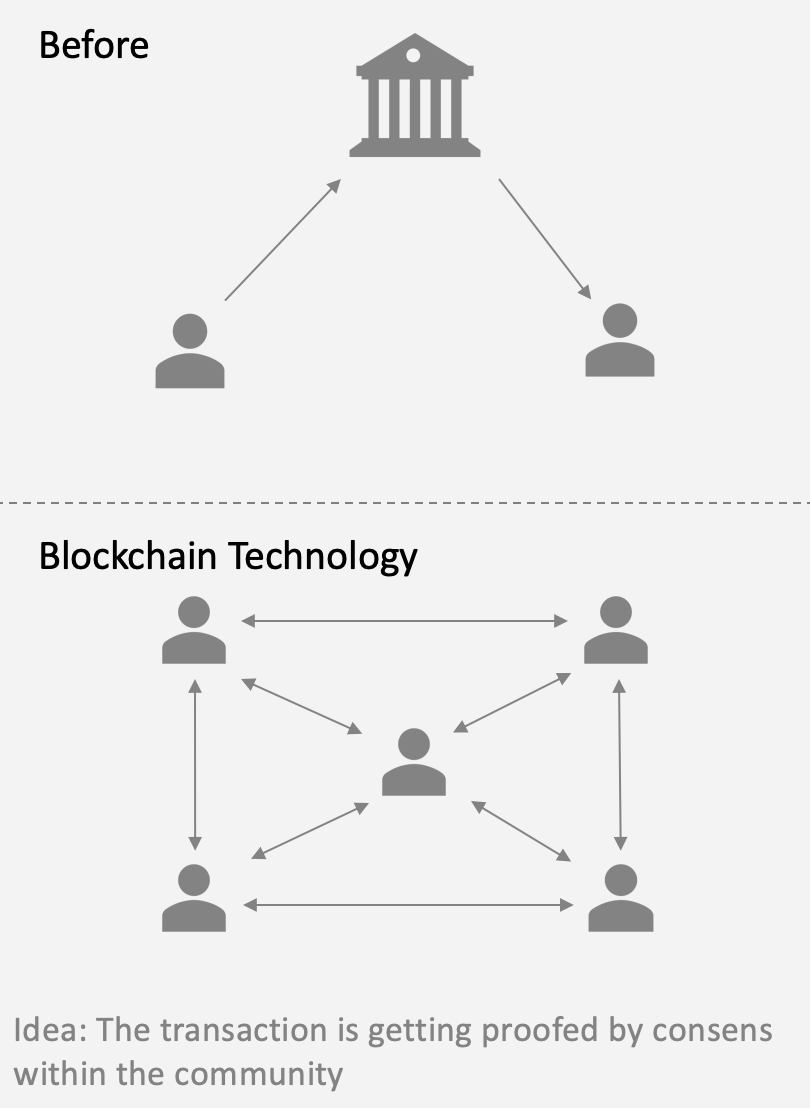
\includegraphics[width=0.485\textwidth, height=300px]{blockchaintech}
\end{figure}

They could realize such a network with three already existing technologies which got combined the first time by Satoshi Nakamoto, for the Bitcoin. 
It describes the whole process how the Bitcoin blockchain gets assembled, validated and agreed for a transaction. 
The blockchain can be assumed as a database that is stored on several computers, in the same version\cite{grishchenko2018semantic}.

The blockchain component can be described as a series of blocks that are combined ordered or chained with each other. 
Everyone stores a variety of information with a hash function.
Were the information in every hash is related to the former one, plus the verification that the transaction is proofed. 
So far, most crypto technology’s work with the so-called proof-of-work \cite{Ray2018}.

The main idea is to find a consent in the network which transactions or blocks are getting approved trough the network. The work part in proof of work relates to the puzzle the community has to solve to verify a transaction and if enough transactions get combined, they can get inserted into a block.

\begin{figure}[ht]
\centering
\caption{How Blocks get chained} 
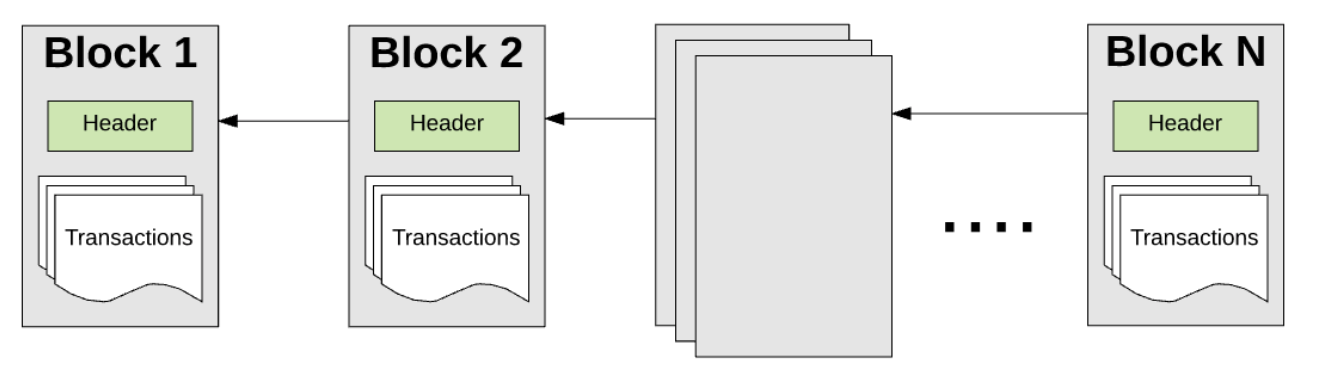
\includegraphics[width=0.45\textwidth]{blockchain}
\end{figure}

% maybe more information about the nonce and the regarding puzzle
This means that transactions can only be verified, if they are gathered and inserted into a newly created block. The person in the network who is creating the new block is called miner and gets compensated with a value for mining. 
The exact compensation depends on the crypto technology. 
In Bitcoin if they verify for the Bitcoin network and in gas if they are mining for the Ethereum Blockchain. 
Every transaction gets collected through it's hash and approved in a block which line up to a chain, so that it gets computationally hard to manipulate a transaction. 
Here one can lead over to the next important component of the bitcoin technology, the peer to peer networks. 

Transferred it means, that there is a network in which each peer is connected to each other without any other intermediary in between.
There is a direct connection between the participants within the network. 
It also is decentralized, such that nobody can manipulate anything.

When the creator of Ethereum thought about this idea and technology, the main question was, what else can be decentralized to cancel trusted intermediaries out and go beyond currencies.
This let Vitalik Buterin in his white paper in late 2013, to describe a platform which can run decentralized applications and therefore run economic systems in pure software. 
The Vision of Ethereum “is to create an unstoppable censorship-resistant self-sustaining decentralized world computer.” [Ray, 2018].
The Ethereum can be explained best, if the dimensions get differentiated into the currency and the platform. 
The platform includes the Ethereum Virtual Machine, the smart contracts and the decentralized applications. 

To add on to the former Bitcoin explanations, the Ethereum is also providing a virtual machine to realize smart contract code. 
Before diving into that topic it should be noted that the Ethereum platform is able to access and alter data to compute anything a turing complete machine could, it is also able to use conditional branches. 
The last requirement to fulfill the turing completeness is to have an arbitrary amount of memory. 
As not all requirements are met the Ethereum virtual machine (EVM) is only quasi-turing complete, because every transaction or computation is requiring a defined amount of gas, that is used to pay the system for mining the blocks. 
The programming language to write applications for the EVM is solidity, which gets compiled to the ‘EVM bytecode’. 
What is the EVM programming language?
The advantage to work on the Ethereum virtual machine allows to make transitions from one state to the other. For example, transactions get executed and gathered into a new block, the new state gets stored and this new block describes the next state.
Here Merkle Patricia trees are used to optimize the verification process of transactions on the EVM [Bisade, 2018].

The mapping between account addresses and the equivalent state of the account has to get stored within the Ethereum platform. That way the data doesn’t need to be sored in a giant block header.
The Merkle Tree structure is thus used to make the hole system scalable. 
In general, a Merkle is following the idea to have a big amount of data which are hashed together. 
They get split into smaller chunk buckets, this gets repeated until there is just a root hash left \cite{Buterin2015}.

\begin{figure*}
  \begin{subfigure}{0.5\textwidth}
    \centering
    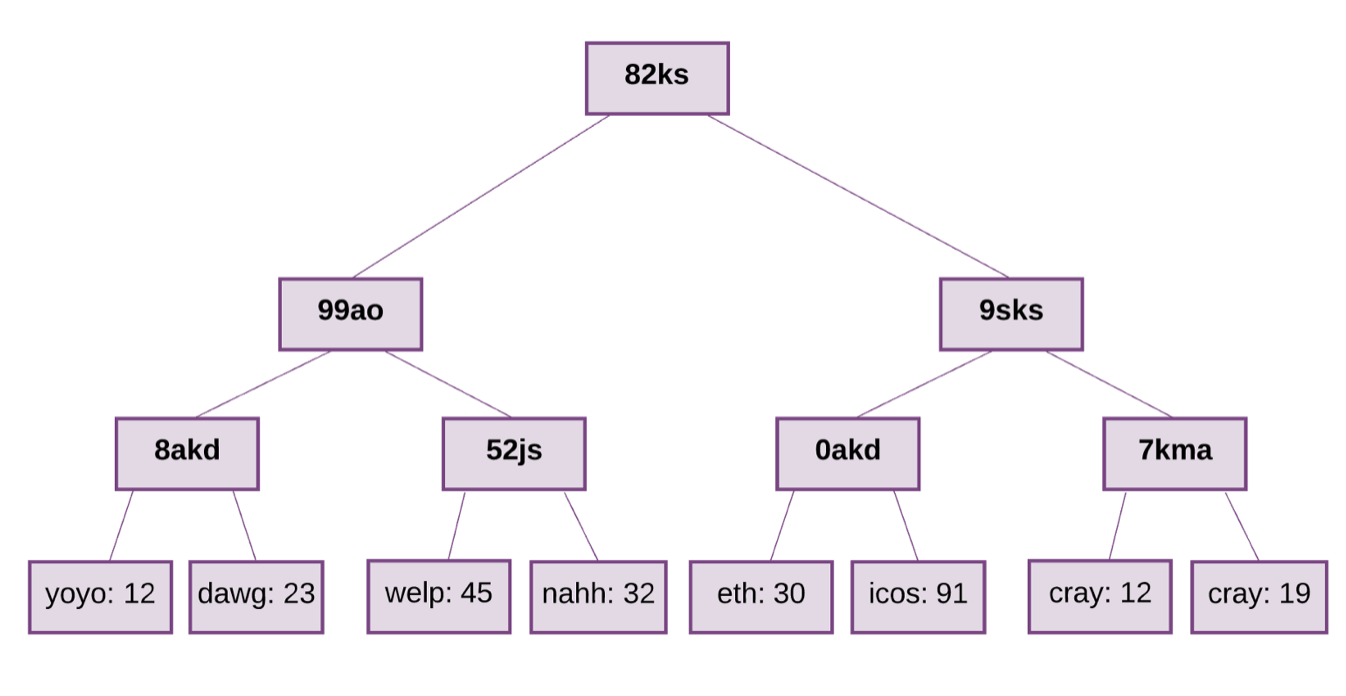
\includegraphics[width=0.9\linewidth]{MerkleTree1.png}
    \caption{Merkle Tree Structure}
  \end{subfigure}%
  \begin{subfigure}{0.5\textwidth}
    \centering
    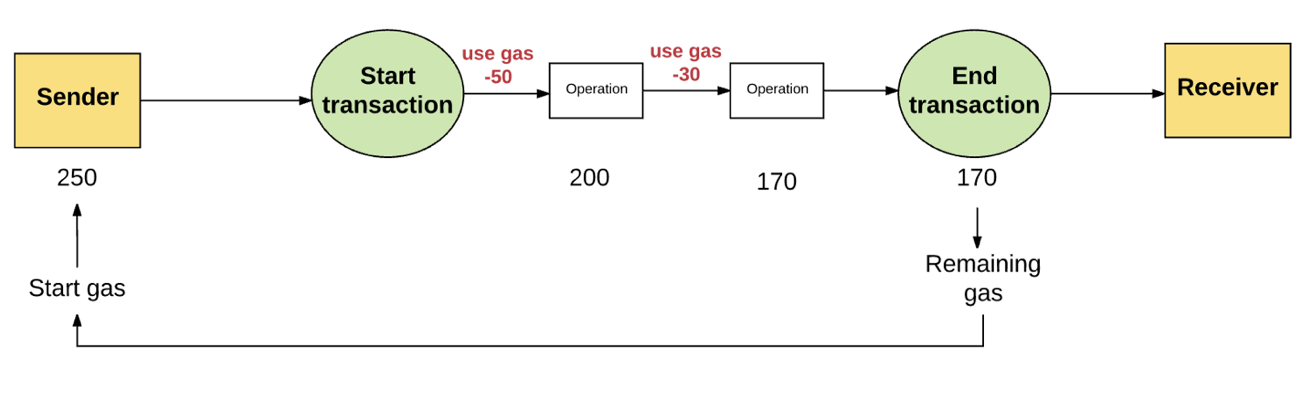
\includegraphics[width=0.7\linewidth, height=120px]{gastransactions.png}
  \caption{Transactions} 
  \end{subfigure}
\end{figure*}

As stated before, this whole process is done to make it possible to perform Merkle proofs. 
They are much quicker and therefore better scalable. 
The proof consists of all the hashes going from the last one up to the root hash, if this get verified by other persons, at least for the verified branch. 
The idea is, that within the database the data is stored in a Merkle tree and the main root is publicly known and proofed. 
If so, a person who wants to get the knowledge about data at a specific position this can be done within less time. 
Because just small amounts of data have to get searched [Buterin, 2015].
This capability to store information in Merkle trees is very useful to improve the scalability and it is called ‘light nodes’. 
So, in the blockchain system exists to types of nodes, full and light ones. 
Whereas the complete one does synchronize the hole chain and is also executing everyone. 
Even though a node does keep every transaction, it is not necessary to store all the data. 
One would just get the header of every transaction done since the first block was mined. 
This system works, because the data is stored in merle trees and can get verified top down. 
In conclusion, the advantages of using such a tree is that the hashes in one tree always dependent on the other hash buckets in the rest of the tree. 
Therefore, if someone wants to manipulate something, it is hard to accomplish. 
As the root hash always keeps information about actual the state, the receipts and the completed transactions, nodes can validate little parts of the chain [Kasireddz 2017].

After giving insights into the processing and storing process in the Ethereum World, the applications on the platform are another important topic.
The Smart contract can be used to run code on the Ethereum Virtual machine in a decentralized way. 
It is comparable to real world contracts. 
A collection of conditions and actions, if a condition occurs, the associated actions are getting executed. 
As a result many real-world applications can be applied to smart contracts. 
The execution happens on the blockchain and is immutable ever after. 
One example often used, is a rent contract in the real work. 
In the real work one would pay rent on a defined date and get entrance to a place for the paid time. A contract represented on Ethereum would look the same, the contracts gets written in Solidity. 
Then the network executes the contract on the defined date and if the renter does pay as expected, means fulfill the condition he gets entrance to his place. If not, the contracts would simply not open the door anymore. 

So, every component of a contract gets represented the enforcement, management and the payment component \cite{Dannen2017IES3103305}.
Back to the example, the person who is renting the property would not get access to his door anymore, if the rent was paid a day later. 
Here the first problem with smart contracts occurs, the rules are really strict, without any room for exceptional circumstances. 
Once the code is executed on the network it cannot be edited or corrected anymore. 
Everything gets executed as written in the code. 
If one does think about complex contracts this can be a problem.
If something gets wrong or if there are paragraphs in it which are not covered by law, with a real contract the law in backing these contracts and one could take out paragraphs after a legal process.
This is not the case in Ethereum, because to edit such a contract the entire network would have to get convinced, that something hast to get changed. Which is almost impossible \cite{Dannen2017IES3103305}.

Ethereum also provides a currency to run and incentivize the previously described system. 
In Ethereum the currency is called Ether. 
To execute and deploy contracts on in the platform and to fulfill the contracts a fee has to get payed.
This will be done in Gas. The concept can be subdivided into gas price and gas. 
The gas-price represents the amount of Ether that one is willing to pay for every unit of gas. 
The subunit of Ether is Wei and is representing the smallest unit. 
The Gas serves as a fee that is required to execute something in the network. 
As shown in the figure, every operation spends the defined amount of gas. 
In case the gas is not enough to fulfill the transactions, the sender ‘runs out of gas’ and the End transaction does not get reached. 


If someone wants to execute something in the network, one has to decide about the gas limit and gas price. 
This has an influence on the amount of computations that one transaction can do.
The miner can collect transactions from the transaction Pool, after they pick them their respective code gets executed on the Virtual Machine and the Merkle proof gets created. 
The last step is to confirm the transaction with the proof of work algorithm. 
The reward depends on the selected amount of gas for the transaction. 
That also means, that some transaction might not get mined in case the fee is chosen to low. Another part the gas is used for, is the storing fee, the amount depends on the size of the storage used \cite{preethi}.
On the one hand this was done, so that people will write optimized and efficient code and won`t waste the Ethereum network computing power on unnecessary tasks \cite{preethi, Dannen2017IES3103305}.
On the other hand, this is a way to incentivize the mining process of transaction. 
This helps to verify the transaction and should be described a little more into detail. 
This process verifies the transaction and is carried out to secure against counterfeiting. 
It is also applying the proof-of-work and uses the Ethereum network, respectively the nodes and creates new blocks with validated transactions. 

The technology also has downsides, one is definitively the scalability. 
Every node in the system is storing the full data and executing every transaction. 
To store the state is a matter of security, also the high degree of decentralization. 
As more traffic gets on the system and more applications get written the data that have to be stored and verified for in the chain, get more and more. 
Specially on the Ethereum platform were there are more then just currency transaction other than the Bitcoin. 
To be comparable to common systems, the Ethereum blockchain has to be able to keep on to the security and decentralization but also work on the scalability. 
So far, the community is working on different alternatives, such as \emph{sharding} and \emph{plasma chains} [Gadaleta 2018].

Vitalik Buterin describes Sharding, combined with Plasma as the most promising solution to make the platform more scalable [Giese 2018].
Here Sharding describes a partition of the main net in smaller shards. 
So far, the blockchain can support 15 transactions per second, with the new solution this could work for 100 transactions afterwards. 
Combined with the plasma solution this could scale up to a million transactions per second. 
The plasma solution represents a second-layer solution could bundle transactions and handle therefore more at ones [Giese 2018].
The main issue always is, that if one wants to higher the scalability, the verifications has to be reduced or less difficult. 
In this triangle one always reducing something, what means the points which have to be manipulated in the network are getting reduced.
Next problem is the high computational power that is needed to verify or mine the transactions, here a lot of energy is needed that the system can work. So far, there is no solution for that.

But with the change to the proof-of-stake this should change.
Besides the scalability and the energy consumption Ethereum has to deal with the high volatility in the crypto market. 
One can imagine, that in case of Ethereum the volatility has an influence on the usage of the platform. 
As described before the currency, called Ether is meant to be the Gas (fee) to pay the system for executing applications. 
If the price went up and down and is opposed by speculation, the original purpose might not get used anymore [Chandersekhar 2018]. 
Chandersekhar looked into the data of Smart Contracts and found out, that 94 \% of the smart contracts are called less then 10 times and just 5 \% are getting called between 10 and 100 times. 
